\documentclass[a4paper, 10pt]{article}

\usepackage{graphicx}
\usepackage{color}
\usepackage{tikz}
\usepackage{pgfplots}
\usepackage{pgf-umlsd}
\usepackage{ifthen}
\usepackage[]{fp}

\FPset{totalOffset}{0}

\begin{document}

\begin{figure}
	\noindent\resizebox{\textwidth}{!}{
	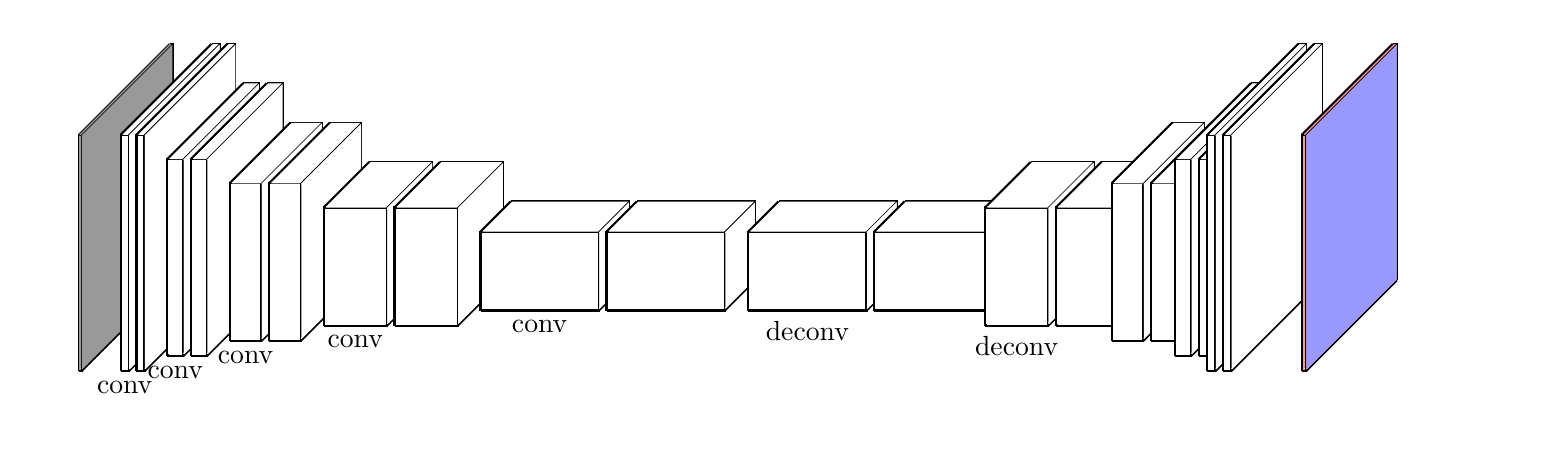
\begin{tikzpicture}
		\draw[use as bounding box, transparent] (-1.8,-1.8) rectangle (17.2, 3.2);

		% Define the macro.
		% 1st argument: Height and width of the layer rectangle slice.
		% 2nd argument: Depth of the layer slice
		% 3rd argument: X Offset --> use it to offset layers from previously drawn layers.
		% 4th argument: Y Offset --> Use it when an output needs to be fed to multiple layers that are on the same X offset.
		% 5th argument: Z Offset -
		% 6th argument: Options for filldraw.
		% 7th argument: Text to be placed below this layer.
		% 8th argument: "start" when you want to reset the offset counter

		\newcommand{\networkLayer}[8]{
			\xdef\totalOffset{\totalOffset}
 			%\ifthenelse{\equal{#8} {start}}
 			%{\FPset{totalOffset}{0}}
 			%{}
 			\FPeval\currentOffset{0+(totalOffset)+(#3)}

			\def\hw{#1} % Used to distinguish input resolution for current layer.
			\def\b{0.02}
			\def\c{#2} % Width of the cube to distinguish number of input channels for current layer.
			\def\x{\currentOffset} % X offset for current layer.
			\def\y{#4} % Y offset for current layer.
			\def\z{#5} % Z offset for current layer.
			%\def\colourOpt{#6}
			\def\inText{#7}

			% Draw the layer body.
			\draw[line width=0.3mm](\c+\x,0+\z,\y) -- (\c+\x,\hw+\z,\y) -- (\x,\hw+\z,\y);                                                      % back plane
			\draw[line width=0.3mm](\x,0+\z,\hw+\y) -- (\c+\x,0+\z,\hw+\y) node[midway,below] {\inText} -- (\c+\x,\hw+\z,\hw+\y) -- (\x,\hw+\z,\hw+\y) -- (\x,0+\z,\hw+\y); % front plane
			\draw[line width=0.3mm](\c+\x,0+\z,\y) -- (\c+\x,0+\z,\hw+\y);
			\draw[line width=0.3mm](\c+\x,\hw+\z,\y) -- (\c+\x,\hw+\z,\hw+\y);
			\draw[line width=0.3mm](\x,\hw+\z,\y) -- (\x,\hw+\z,\hw+\y);
			
			% Recolor visible surfaces
			\filldraw[#6] (\x+\b,\b+\z,\hw+\y) -- (\c+\x-\b,\b+\z,\hw+\y) -- (\c+\x-\b,\hw-\b+\z,\hw+\y) -- (\x+\b,\hw-\b+\z,\hw+\y) -- (\x+\b,\b+\z,\hw+\y); % front plane
			\filldraw[#6] (\x+\b,\hw+\z,\hw-\b+\y) -- (\c+\x-\b,\hw+\z,\hw-\b+\y) -- (\c+\x-\b,\hw+\z,\b+\y) -- (\x+\b,\hw+\z,\b+\y);
			
			% Colored slice.
			\ifthenelse {\equal{\inText} {}}
			{} % Do not draw colored slice if #4 is blank.
			{\filldraw[#6] (\c+\x,\b,\hw-\b+\y) -- (\c+\x,\b,\b+\y) -- (\c+\x,\hw-\b,\b+\y) -- (\c+\x,\hw-\b,\hw-\b+\y);} % Else, draw a colored slice.
			{\filldraw[#6] (\c+\x,\b+\z,\hw-\b+\y) -- (\c+\x,\b+\z,\b+\y) -- (\c+\x,\hw-\b+\z,\b+\y) -- (\c+\x,\hw-\b+\z,\hw-\b+\y);} % Else, draw a colored slice.
			
			\FPeval\totalOffset{0+(currentOffset)+\c}
		}

		% INPUT
		\networkLayer{3.0}{0.03}{0.0}{0.0}{0.0}{color=gray!80}{}{start}

		% ENCODER
		\networkLayer{3.0}{0.1}{0.5}{0.0}{0.0}{color=white}{conv}{}    % S1
		\networkLayer{3.0}{0.1}{0.1}{0.0}{0.0}{color=white}{}{}        % S2
		\networkLayer{2.5}{0.2}{0.1}{0.0}{0.0}{color=white}{conv}{}    % S1
		\networkLayer{2.5}{0.2}{0.1}{0.0}{0.0}{color=white}{}{}        % S2
		\networkLayer{2.0}{0.4}{0.1}{0.0}{0.0}{color=white}{conv}{}    % S1
		\networkLayer{2.0}{0.4}{0.1}{0.0}{0.0}{color=white}{}{}        % S2
		\networkLayer{1.5}{0.8}{0.1}{0.0}{0.0}{color=white}{conv}{}    % S1
		\networkLayer{1.5}{0.8}{0.1}{0.0}{0.0}{color=white}{}{}        % S2
		\networkLayer{1.0}{1.5}{0.1}{0.0}{0.0}{color=white}{conv}{}    % S1
		\networkLayer{1.0}{1.5}{0.1}{0.0}{0.0}{color=white}{}{}        % S2

		% DECODER
		\networkLayer{1.0}{1.5}{0.3}{0.0}{0.0}{color=white}{deconv}{} % S1
		\networkLayer{1.0}{1.5}{0.1}{0.0}{0.0}{color=white}{}{}       % S2
		\networkLayer{1.5}{0.8}{0.1}{0.0}{0.0}{color=white}{deconv}{} % S1
		\networkLayer{1.5}{0.8}{0.1}{0.0}{0.0}{color=white}{}{}       % S2
		\networkLayer{2.0}{0.4}{0.1}{0.0}{0.0}{color=white}{}{}       % S1
		\networkLayer{2.0}{0.4}{0.1}{0.0}{0.0}{color=white}{}{}       % S2
		\networkLayer{2.5}{0.2}{0.1}{0.0}{0.0}{color=white}{}{}       % S1
		\networkLayer{2.5}{0.2}{0.1}{0.0}{0.0}{color=white}{}{}       % S2
		\networkLayer{3.0}{0.1}{0.1}{0.0}{0.0}{color=white}{}{}       % S1
		\networkLayer{3.0}{0.1}{0.1}{0.0}{0.0}{color=white}{}{}       % S2

		% OUTPUT
		\networkLayer{3.0}{0.05}{0.9}{0.0}{0.0}{color=red!40}{}{}          % Pixelwise segmentation with classes.
		\networkLayer{3.0}{0.05}{-0.05}{0.0}{7.0}{color=blue!40}{For Z}{}


	\end{tikzpicture}
	}
	\caption{Example CNN.}
	\label{fig:cnn}
\end{figure}

\end{document}
